\chapter{Example Algorithm}

An example algorithm for compressed branch trace is given in figure \ref{fig:algo}. In the diagram, {\textit {unprediscon}} is short for unpredictable discontinuity; when the program counter changes in a manner that cannot be predicted from the source code alone. {\textit {te\_inst}} is the name of a type of packet emitted by the encoder. 

\textit{Context} is a generic term that refers to the threadID. This could be the HART ID and/or the software context id. This is reported when there is a change.

\begin{figure}[l]
\begin{center}
  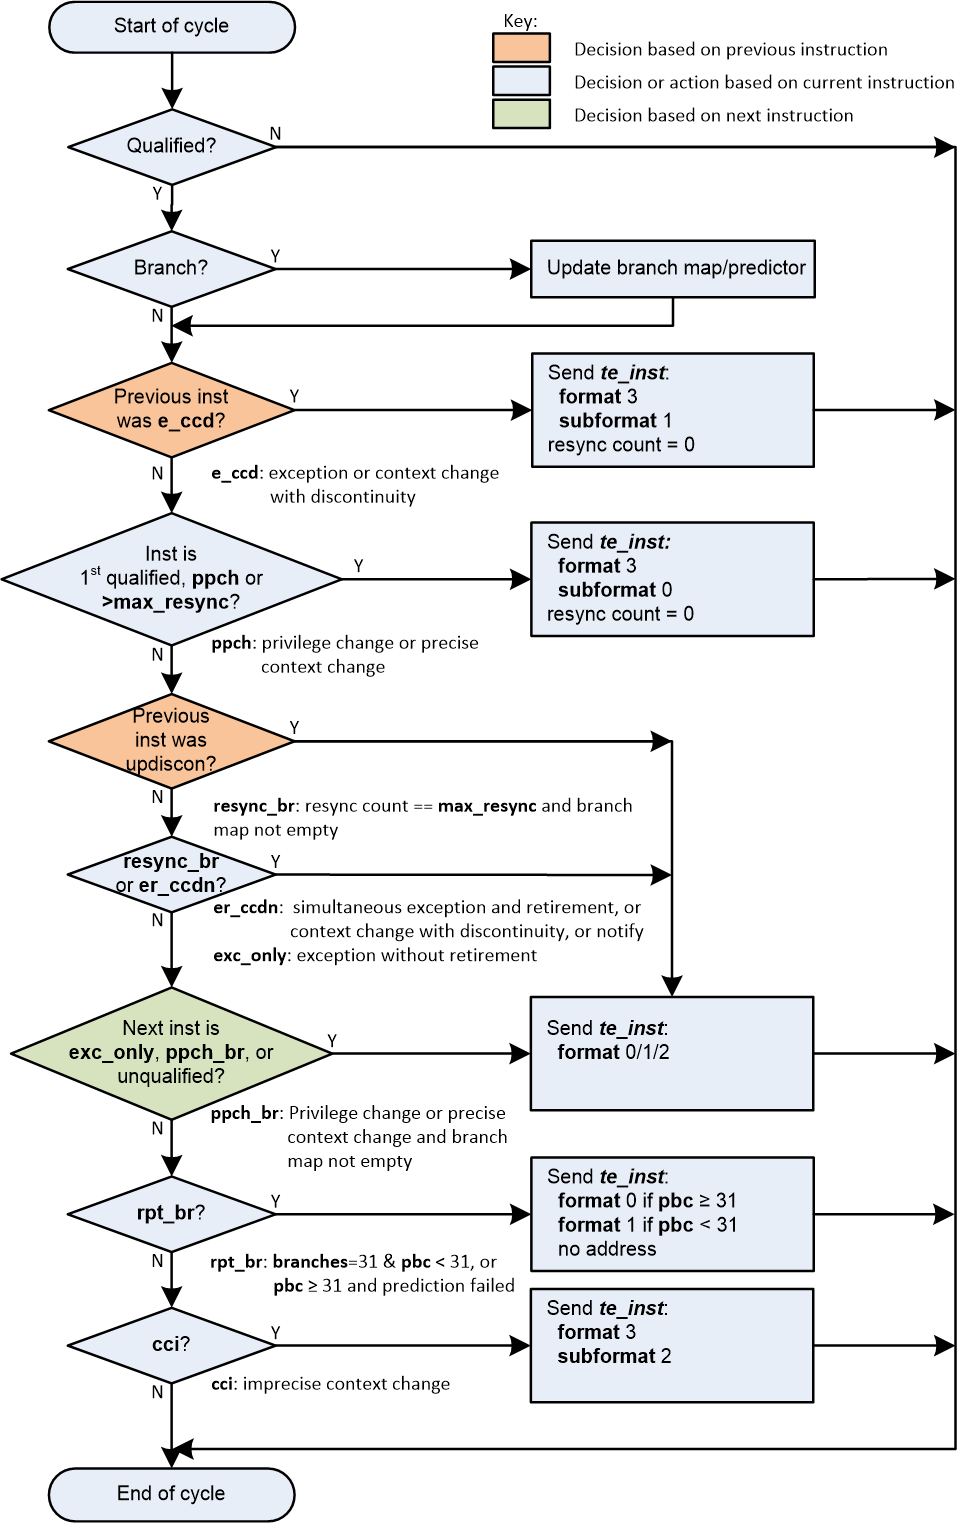
\includegraphics[height=23cm, width=15cm]{algo.png}
  \caption{Delta Mode 1 instruction trace algorithm}
  \label{fig:algo}
\end{center}
\end{figure}


